\documentclass[crop,tikz]{standalone}

\usetikzlibrary{arrows}
\usetikzlibrary{positioning}

\begin{document}
  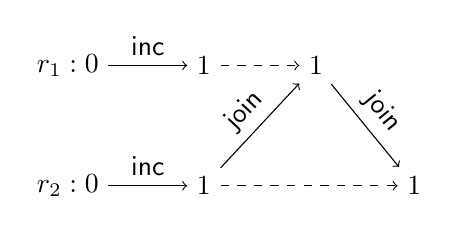
\begin{tikzpicture}
    \node (r1a) {$r_1:0$};
    \node (r2a) [below = of r1a] {$r_2:0$};

    \node (r1b) [right = of r1a] {$1$};
    \node (r2b) [right = of r2a] {$1$};

    \node (r1c) [right = of r1b] {$1$};
    \node (r2c) [right = of r2b] {};
    \node (r2d) [right = of r2c] {$1$};

    \draw [->] (r1a) -- node [above] {\textsf{inc}} (r1b);
    \draw [->] (r2a) -- node [above] {\textsf{inc}} (r2b);

    \draw [->,dashed] (r1b) -- (r1c);
    \draw [->] (r2b) -- node [midway, sloped, above] {\textsf{join}} (r1c);

    \draw [->,dashed] (r2b) -- (r2d);
    \draw [->] (r1c) -- node [midway, sloped, above] {\textsf{join}} (r2d);
  \end{tikzpicture}
\end{document}
